% This section should describe the overall structure of your software system. Think of it as the strategy for how you will build the system. An architectural "layer" is the top-level logical view, or an abstraction, of your design. Layers should be composed of related elements of similar capabilities, and should be highly independent of other layers, but should have very clearly defined interfaces and interactions with other layers. Each layer should be identified individually and should be unique as to its function and purpose within the system. This section should also contain the high-level block diagram of the layers, as shown in the example below, as well as detailed descriptions of the functions of each layer.

%%%%%%%%%%%%%%%%%%%%%%%%%%%%%%%%%%%%%%%%%%%%%%%%%%%%%%%%%%%%%%%%%%%%%%%%%%%%
%   Change the graphic here. Put your image in the 'images' folder
%   and update the name from 'images/test_image' to your image name
\begin{figure}[h!]
	\centering
 	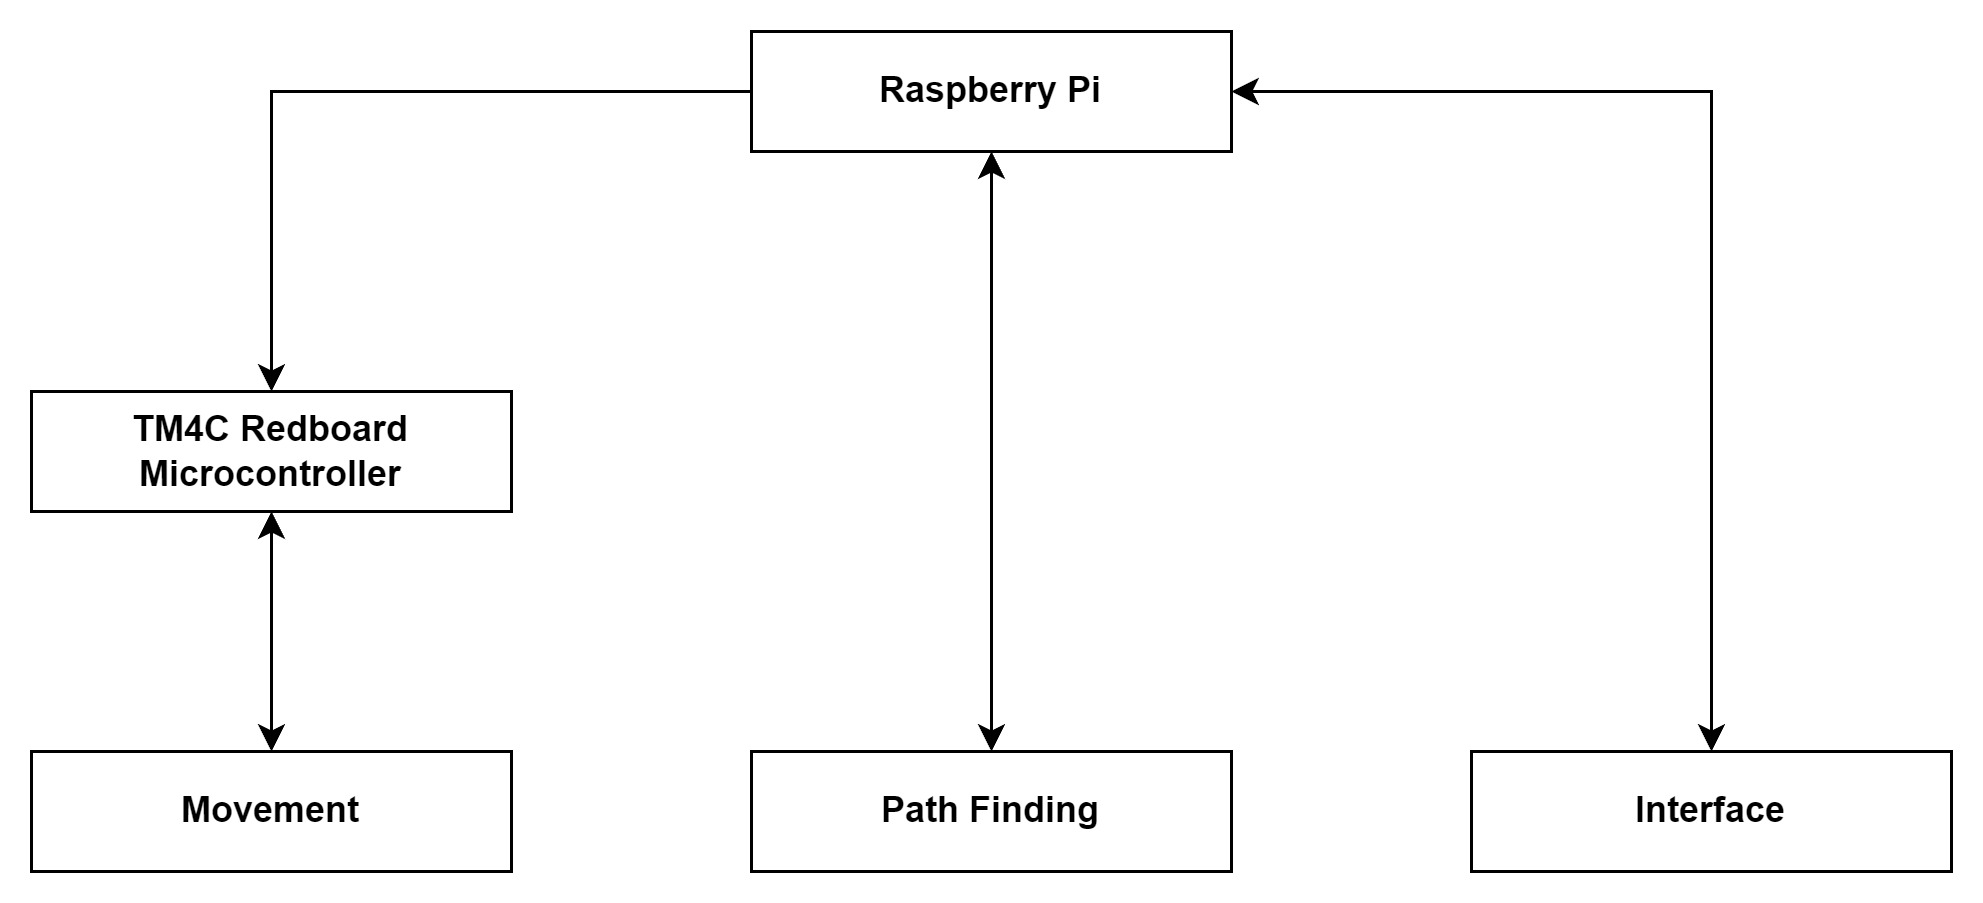
\includegraphics[width=0.60\textwidth]{images/layers}
 \caption{A simple architectural layer diagram} % Be sure to change the caption!
\end{figure}

\subsection{Movement - Description}
%Each layer should be described separately in detail. Descriptions should include the features, functions, critical interfaces and interactions of the layer. The description should clearly define the services that the layer provides. Also include any conventions that your team will use in describing the structure: naming conventions for layers, subsystems, modules, and data flows; interface specifications; how layers and subsystems are defined; etc. 
The movement layer of the Roam\_Bot is responsible for facilitating the rover's movement including the crash prevention feature, odometer, speed, and direction control. All instructions in this layer pass through Motor\_Control using PWM and GPIO. The speed and direction subsystems both use PWM to achieve a user-provided speed and the algorithm determines the direction. The crash\_prevention and odometer subsystems both use GPIO to let the rover know when to stop.

\subsection{Path Finding - Description}
%Each layer should be described separately in detail. Descriptions should include the features, functions, critical interfaces and interactions of the layer. The description should clearly define the services that the layer provides. Also include any conventions that your team will use in describing the structure: naming conventions for layers, subsystems, modules, and data flows; interface specifications; how layers and subsystems are defined; etc. 
The path-finding layer of the Roam\_Bot is responsible for the navigation of the rover. This layer communicated with a TM4C to facilitate communication with the LIDAR. LIDAR will be used in the navigation to create a mapping of the room and communicate obstacles. The LIDAR and navigation will use UART.

\subsection{Interface - Description}
%Each layer should be described separately in detail. Descriptions should include the features, functions, critical interfaces and interactions of the layer. The description should clearly define the services that the layer provides. Also include any conventions that your team will use in describing the structure: naming conventions for layers, subsystems, modules, and data flows; interface specifications; how layers and subsystems are defined; etc.
The user interface layer is responsible for receiving user input. This layer is made up of 3 subsystems. The starting UI will display and redirect the user to algorithm upload or user control. User Control will use UART to accept rover commands. The algorithm upload uses UART to read a file into the system. 